\subsection{Функціональні вимоги}
\subsubsection*{Тезаурус}

\begin{description}
\setlength{\itemsep}{0pt}
\item[Курс] --- послідовність занять з певної дисципліни у певний період з певним набором слухачів.
\item[Оператор] --- особа, що займається записом слухачів, внесенням курсів у систему, прийомом оплат та формуванням звітів.
\item[Слухач] --- особа, що відвідує курс.
\item[Звіт] --- паперовий чи електронний документ, що містить зведену інформацію про курси.
\item[Розклад] --- перелік дат та часу проведення занять зі вказанням типу заняття та місця його проведення.
\item[Заняття] --- одна урочна година.
\item[Заявка] --- вияв наміру потенційного слухача сплачувати та відвідувати курс.
\item[Коефіціент] --- множник, що використовується при автоматичному розрахунку зарплати викладача і вартості курсу, що залежить від неї.
\item[Сповіщення] --- текстова нотатка, що інформує користувача системи про якусь подію і дозволяє вибрати щодо неї певну дію.
\item[Форма договору] --- бланк документу, що затверджує зобов'язання кафедри СПЗ провести для слухача курс, а слухача --- сплатити курс.
\item[Оплата] --- разове внесення коштів за курс, може не покривати вартість курсу повністю.
\item[Заборгованість] --- різниця між вартість курсу та сумою сплачених слухачем за курс коштів.

\subsubsection*{Класифікація функціональних вимог (з аналізом за принципом MoSCoW)}
\begin{itemize}
 \item Життєвий цикл
 \begin{itemize}
  \item Організаційні процеси
  \begin{itemize}
   \item Навчання
   \begin{itemize}
    \item Опанування Kendo UI
   \end{itemize}
   \item Створення інфраструктури
   \item Керування проектом
  \end{itemize}
  \item Основні процеси
  \begin{itemize}
   \item Розробка
   \begin{itemize}
    \item Аналіз вимог
    \item {[}M{]} ВВ: реєстрація
    \item {[}M{]} ВВ: авторизація
    \item {[}M{]} ВВ: робота з викладачами
    \item {[}M{]} ВВ: робота з курсами
    \item {[}W{]} ВВ: робота з розкладом
    \item {[}M{]} ВВ: робота зі слухачами
    \item {[}M{]} ВВ: запис слухачів на курс
    \item {[}M{]} ВВ: робота з обліковими записами
    \item {[}C{]} ВВ: робота з коефіціентами
    \item {[}S{]} ВВ: створення звітів
    \item {[}S{]} ВВ: обробка заявок
    \item {[}M{]} ВВ: обробка облікових записів
   \end{itemize}
   \item Впровадження
  \end{itemize}
  \item Допоміжні процеси
  \begin{itemize}
   \item Документування
   \item Забезпечення якості
   \begin{itemize}
    \item Модульне тестування
    \item Тестування інтерфейсу користувача
   \end{itemize}
   \item Вирішення проблем
  \end{itemize}
 \end{itemize}
\end{itemize}
\end{description}

\subsection{Нефункціональні вимоги}
\begin{itemize}
 \item Відображати та редагувати дані, що вводяться в систему, у таблицях
 \item Відображати на екрані одну або дві різні таблиці одночасно
 \item Вкладені таблиці для сутностей, пов'язаних зв'язком M--M
 \item Гарячі клавіші для додання нового запису, видалення запису, збереження запису
 \item Підтримка стабільних версій браузерів Firefox та Chrome, Internet Explorer 8--11
 \item Час реакції $\leqslant$ 5 секунд
 \item Імовірність збою --- 0.01
 \item Підтримка резервного копіювання даних та відновлення з резервних копій
\end{itemize}

\subsection{Планування розробки}
Представлення: клієнт. Бізнес-логіка: сервер. Дані: БД.

Технології розробки: мова PHP5.4, СКБД MySQL 5, Web-технології, формат даних JSON.

Інструменти розробки: редактор Vim, система контролю версій Git, бібліотека тестування запитів Dogpatch.

Діаграми: рис. 1--3.

\begin{landscape}
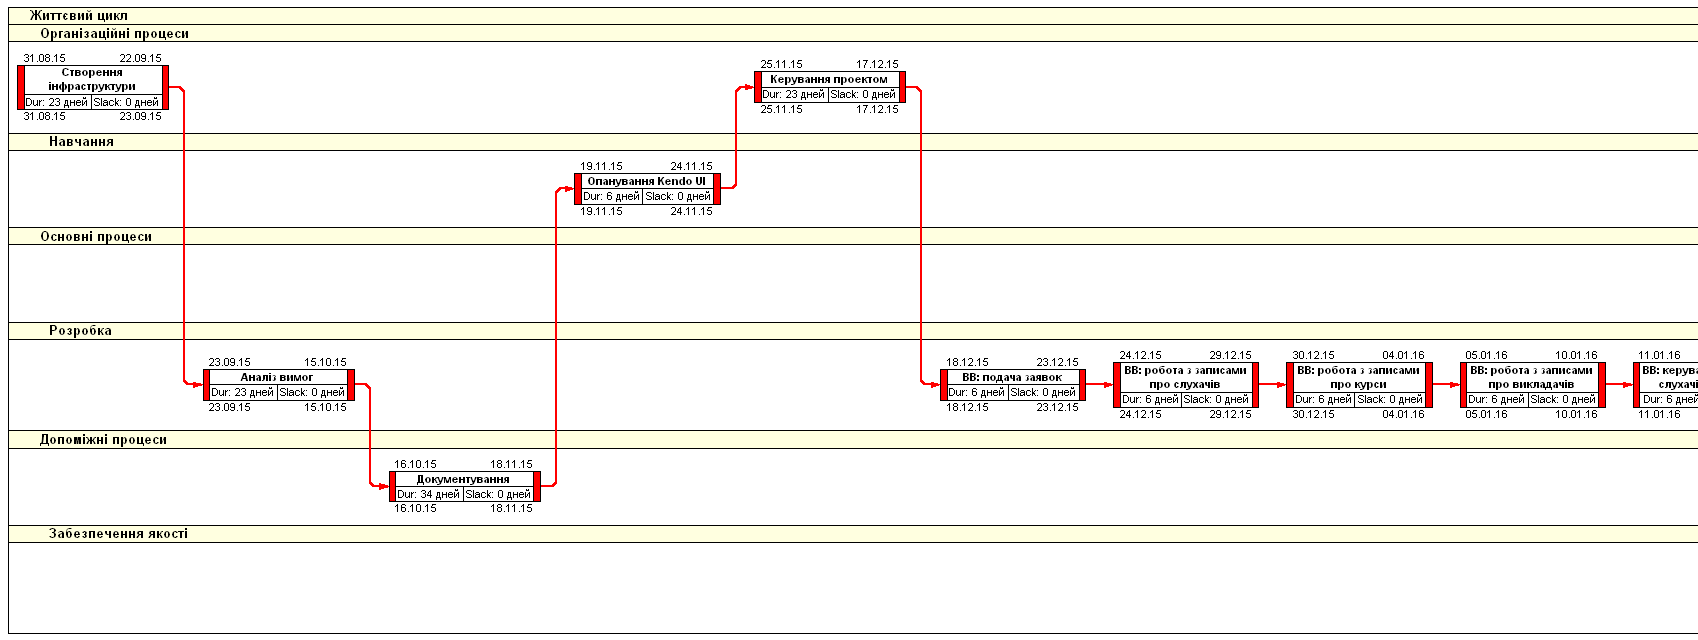
\includegraphics[width=24cm]{smp_cgw2_2.png}\\
\imglabel{Діаграма WBS}
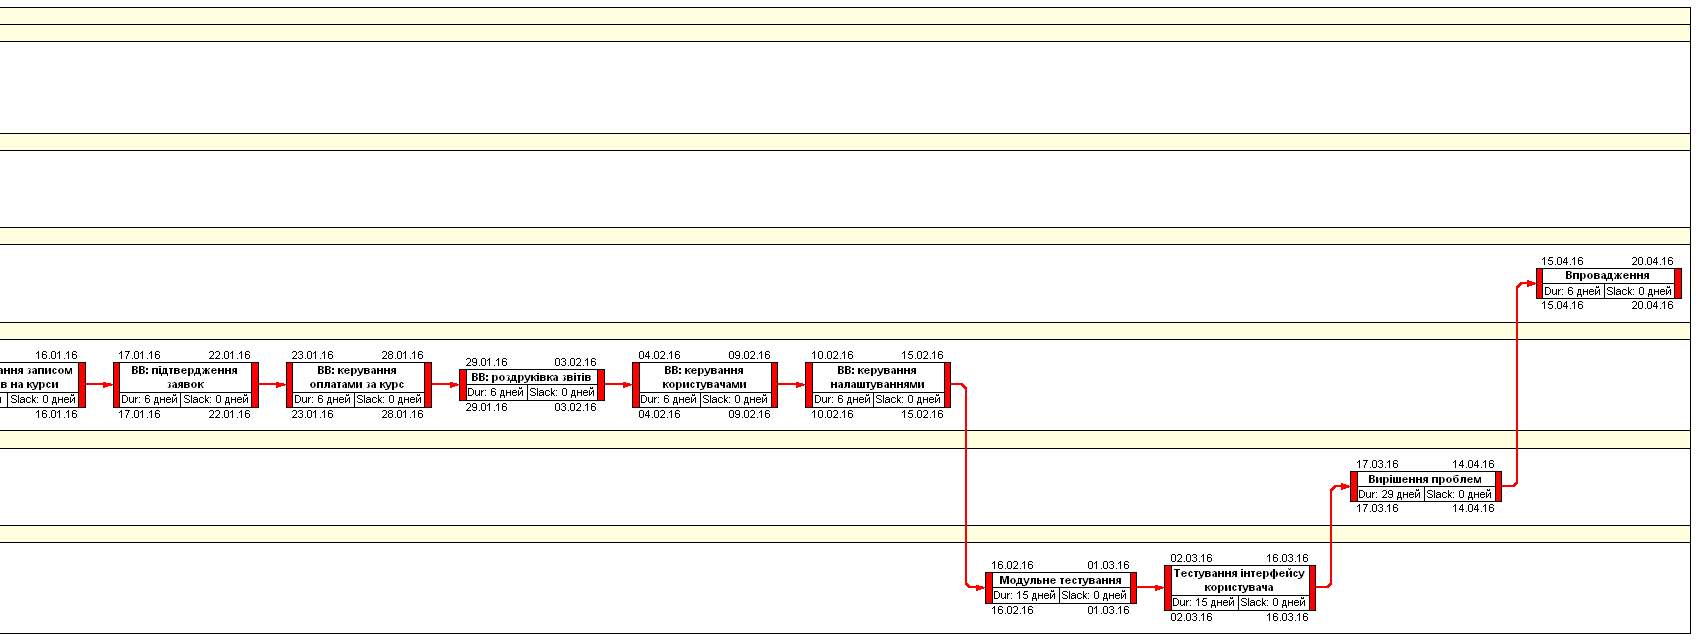
\includegraphics[width=24cm]{smp_cgw2_3.png}\\
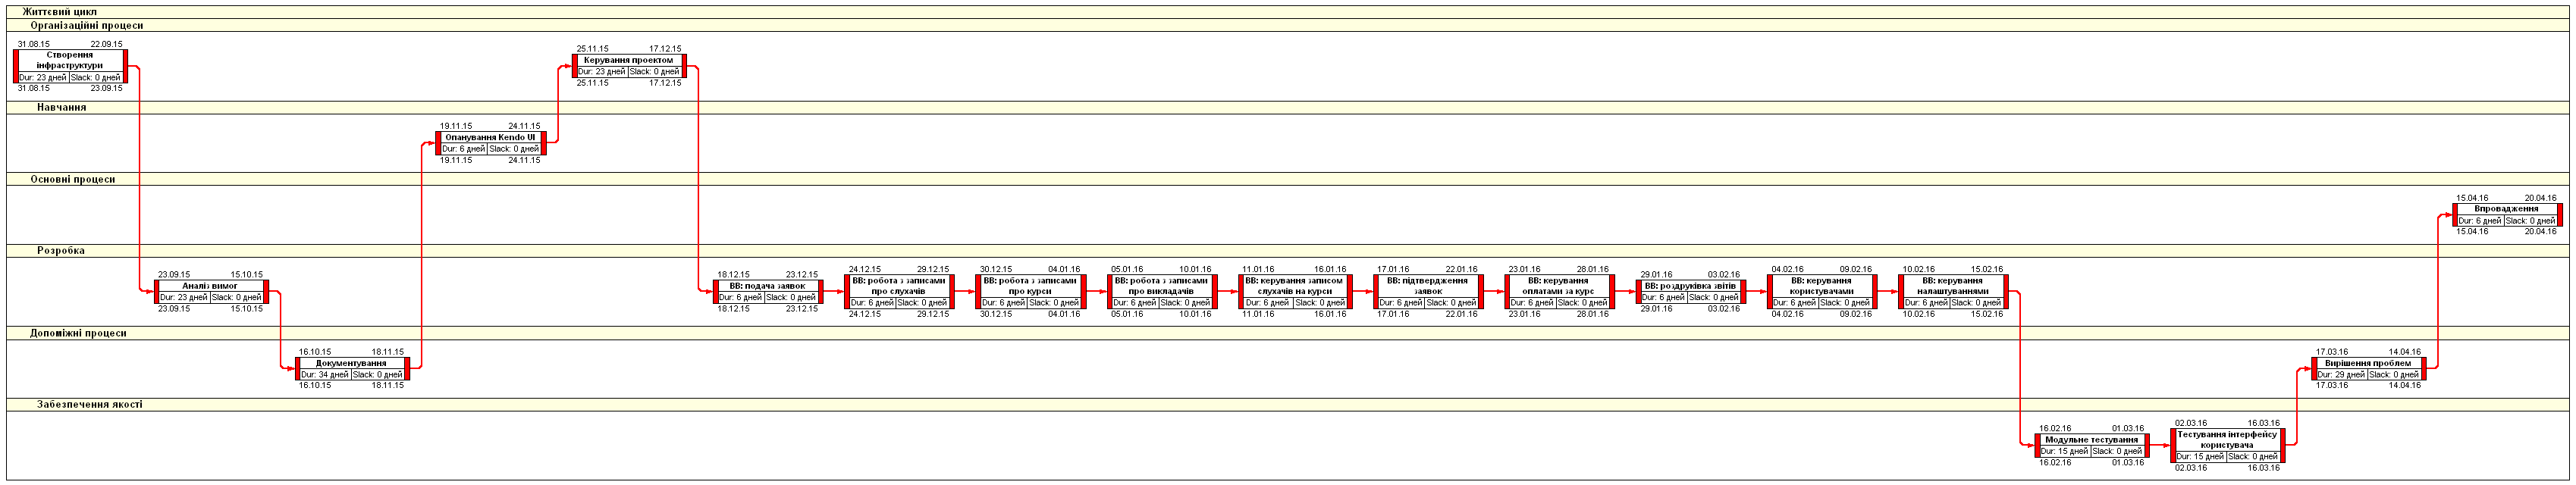
\includegraphics[width=24cm]{smp_cgw2_4.png}
\imglabel{Діаграма WBS (продовження)}
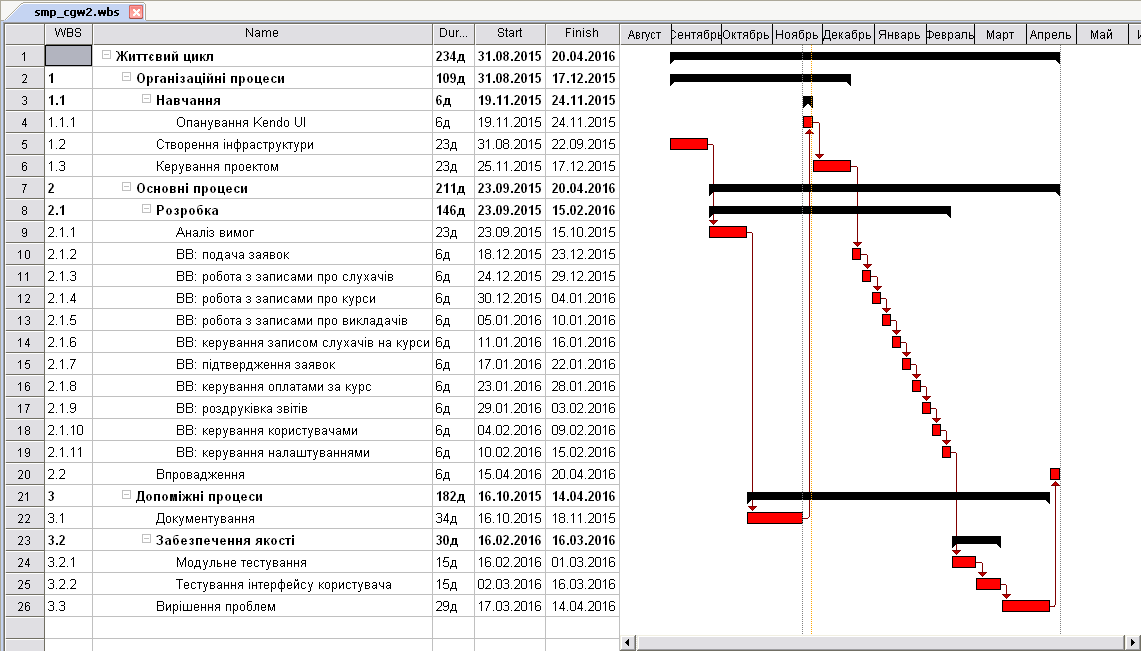
\includegraphics[width=24cm]{smp_cgw2_1.png}
\imglabel{Діаграма Ганта}
\end{landscape}
